\documentclass[12pt]{article}
\usepackage{sbc-template}
\usepackage{graphicx,url}
\usepackage{float}
\usepackage[brazil]{babel}   
\usepackage[utf8]{inputenc}  
\usepackage{url}
\bibliographystyle{ieeetr}

\usepackage{inconsolata}

\usepackage{color}

\definecolor{pblue}{rgb}{0.13,0.13,1}
\definecolor{pgreen}{rgb}{0,0.5,0}
\definecolor{pred}{rgb}{0.9,0,0}
\definecolor{pgrey}{rgb}{0.46,0.45,0.48}

\usepackage{listings}
\lstset{language=Java,
	showspaces=false,
	showtabs=false,
	breaklines=true,
	showstringspaces=false,
	breakatwhitespace=true,
	commentstyle=\color{pgreen},
	keywordstyle=\color{pblue},
	stringstyle=\color{pred},
	basicstyle=\ttfamily
}
     

\sloppy
	\title{ Simulação de Pool de Impressão Dístribuida Utilizando Socket \\ Exercício Computacional II - Sistemas Distribuídos}

\author{Rafael Gonçalves de Oliveira Viana\inst{1}  }


\address{Sistemas de Informação -- Universidade Federal do Mato Grosso do Sul
	(UFMS)\\
  	Caixa Postal 79400-000 -- Coxim -- MS -- Brazil
  \email{rafael.viana@aluno.ufms.br }
  \\\vspace*{10pt} \normalsize  \today{}
}

\begin{document} 

\maketitle

     
\begin{resumo} 	
  Este relatório introduz a arquitetura de uma Pool de Thread.
\end{resumo}

\section{Introdução}
 De acordo com \cite{entf} em um ambiente de trabalho, onde deseja se imprimir documentos enviados num curto período de tempo, nessecita se  utilizar o pool de impressão.
 
 Uma pool de impressão permite que várias impressoras físicas possam ser controladas por uma única impressora lógica,  sempre que um trabalho for enviado para a impressora lógica, esta consultará o estado das impressoras físicas para verificar qual equipamento está livre no momento e enviará o trabalho para ela .
 
\section{Fundamentação Téorica} 
	Nesta sessão serão tradatas, as tecnologias que foram utilizadas neste documento, como é o exemplo das bibliotecas Java  Sockets e Threads.
 
\subsection{Socket}
 Segundo \cite{socket}.\cite{conc}.
 Os sockets são compostos por um conjunto de primitivas do sistema operacional e foram originalmente desenvolvidos para o BSD Unix. Podem ser utilizados nos mais variados sistemas operacionais com recursos de comunicação em rede, sendo suportados pela maioria das linguagens de programação. Sockets são suportados em Java desde o JDK 1.0, para sua utilização devemos fazer uso das classes contidas no pacote java.net. Um exemplo interessante da programação de sockets em Java são os drivers JDBC do tipo 4, que usam sockets para comunicar-se diretamente com a API de rede do banco de dados.
 
\begin{figure}[H]
	\centering
	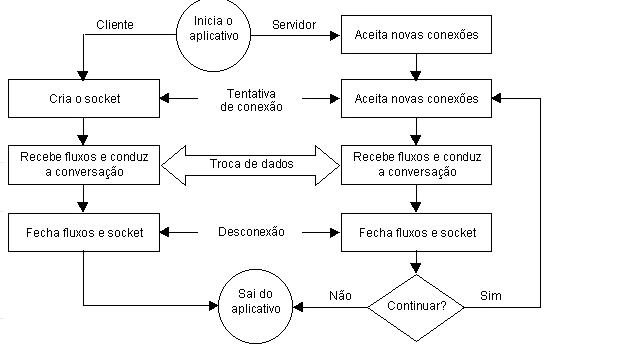
\includegraphics[scale=1]{imagens/fluxoSocket.JPG}
    \caption{Fluxo de troca de dados com sockets.}
	\label{fluxoSocket}
\end{figure}
 \begin{lstlisting}
 /**
 * This is a doc comment.
 */
public void executa() throws IOException {
	Buffer.addImpressora(new Impressora("127.0.0.1",2323,"2323"));
	Buffer.addImpressora(new Impressora("127.0.0.1",2324,"2324"));
	SaidaDocumento escalonador = new SaidaDocumento();
	new Thread(escalonador).start();
	ServerSocket servidor = new ServerSocket(this.porta);
	System.out.println("Porta "+porta+" aberta!");
	while (true) {
		Socket cliente = servidor.accept();
	      ChegadaDocumento tc = new ChegadaDocumento(cliente, new 		 Scanner(cliente.getInputStream()).nextLine(),
		new PrintStream(cliente.getOutputStream()));
		new Thread(tc).start();
	}

}
 \end{lstlisting}
 
\subsection{ Threads -  Problema de Concorrência}
 Da necessidade de dois computadores se comunicarem, surgiram diversos protocolos que permitissem tal troca de informação: o protocolo que vamos usar aqui é o TCP (Transmission Control Protocol) \cite{conc}.

\begin{figure}[H]
	\centering
	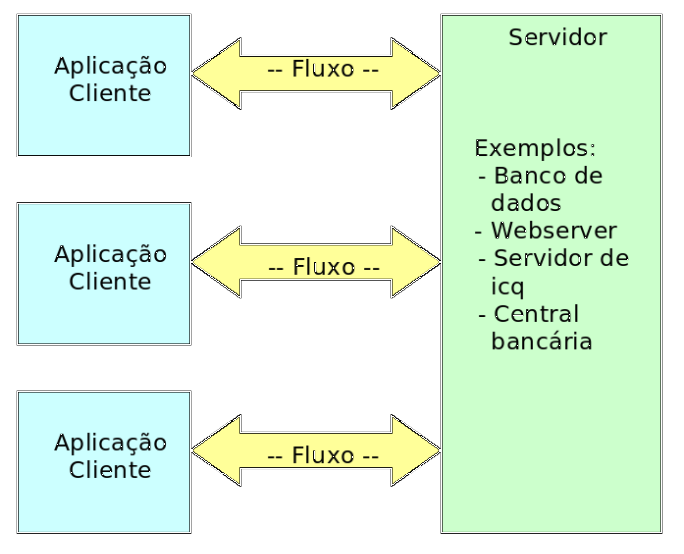
\includegraphics[scale=0.14]{imagens/fluxo.png}
	\caption{Conexão TCP.}
	\label{fluxotcp}
\end{figure} 
É possível conectar mais de um cliente ao mesmo servidor, como é o caso de diversos banco de dados, servidores Web, etc.

\section{Desenvolvimento}
Para resolver o trabalho proposto, foi desenvolvido uma aplicação java que simula, uma pool de impressões que as ordena e envia para uma impressora.
	Foram criadas 3 classes Javas sendo elas Cliente, Pool de Impressão e Impressora as mesmas serão comentandqas nas póximas sessões
	
\subsection{Clientes}
	Essa classe  se conecta a classe servidor com objetivo de repassar informações via Socket, que serão processadas posteriormente notificando o cliente do processamento da impressão.
	



\subsection{Pool de Impressão}\label{pool}
  Classe responsável pela comunicação dos Sockets (Cliente/Impressora), esse como as demais e de extrema importancia para o desenvolverdos.


\subsection{Impressoras}
	Classe responsável pela impressão dos documentos contidos  no buffer da Pool de Impressão \ref{pool}.
	Ela é notificada pelo escalonador de impressões de que novos documentos chegaram, e que os mesmos podem ser impressos .


\section{Conclusão}
Neste relatório foi apresentado a estrutura básica de um.


\bibliography{bibli}

\end{document}


